\documentclass[11pt]{article}
\usepackage[utf8]{inputenc}
\usepackage[T1]{fontenc}
\usepackage{grffile}
\usepackage{longtable}
\usepackage{wrapfig}
\usepackage{rotating}
\usepackage[normalem]{ulem}
\usepackage{amsmath}
\usepackage{textcomp}
\usepackage{amssymb}
\usepackage{capt-of}
\usepackage{hyperref}
\hypersetup{colorlinks=true, linkcolor=magenta, citecolor=cyan}
\setlength{\parindent}{0in}
\usepackage[margin=1in]{geometry}
\usepackage[english]{babel}
\usepackage{mathtools}
\usepackage{palatino}
\usepackage{fancyhdr}
\usepackage{sectsty}
\usepackage{engord}
\usepackage{parskip}
\usepackage{minted}
\usepackage{graphicx}
\usepackage{subcaption}
\usepackage{setspace}
%\usepackage[center]{caption}
\usepackage{placeins}
\usepackage{color}
\usepackage{amsmath}
\usepackage{bm}
\usepackage{todonotes}
\usepackage{pdfpages}
% \titlespacing*{\subsection}{0pt}{5.5ex}{3.3ex}
%\titlespacing*{\section}{0pt}{5.5ex}{1ex}
\usepackage{natbib}

\author{Luis Antonio Ortega Andrés\\Antonio Coín Castro}
\date{\today}
\title{DeepFakes Detection Lab - Report}
\hypersetup{
 pdfauthor={Luis Antonio Ortega Andrés, Antonio Coín Castro},
 pdftitle={},
 pdfkeywords={},
 pdfsubject={},
 pdflang={Spanish}
 }

\begin{document}

\maketitle

\section*{Task 1: intra-database analysis}

\textit{The goal of this task is to develop and evaluate DeepFake detection systems over the same database. In this task, you should use only the UADFV database, which is divided into \texttt{development} and \texttt{evaluation} datasets.}

\textbf{a)} \textit{Provide all details (including links or references if needed) of your proposed DeepFake detection system.}

\textbf{b)} \textit{Provide all details of the development/training procedure followed and the results achieved using the development dataset of the UADFV database. Show the results achieved in terms of Receiver Operating Characteristic (ROC) curve and Area Under the Curve (AUC).}

\textbf{c)} \textit{Describe the final evaluation of your proposed DeepFake detection system and the results achieved using the evaluation dataset (not used for training). Show the results achieved in terms of ROC curve and AUC. Provide an explanation of your results.}

First of all, we are reviewing the followed training procedure along with the acquired results at test evaluations. Secondly, all the approaches that have being considered will be summarized with their reasons for being discarded.

\subsection*{Preprocessing}

Let us begin with the preprocessing procedure, for both training and test datasets, the given images from UADFV have been preprocessed following these steps:
\begin{enumerate}
  \item We use MTCNN face detector (\cite{zhang2016joint}) in order to crop the section of the image that contains the face. The aim of this phase is to erase those parts of the image that are not relevant for our classification task.
  \item We used \texttt{dlib} (\cite{dlib09}) in order to retrieve landmarks from face images. With this method, the \( (x,y) \) position of \( 68 \) landmarks is generated per sample image.
  \item We add random noise to the image, more precisely, we randomly decide wether the image is slightly blurred using a GaussianBlur filter from OpenCV (\cite{opencv_library}) or it is perturbed using Gaussian noise. Each of the procedures is equally probable and every image goes through one or the other but never both. The aim is this procedure is to add some regularization to the learning method, as a result, this is only applied to training samples, that is, validation and test are not perturbed.
  \item The face image is transformed into a gray-scale image and the intensity of such gray is retrieved from the landmarks retrieved by \texttt{dlib}.
  \item The feature vector of each image is composed by each landmark intensity, this results in 68 features for each image.
\end{enumerate}

From the procedure described above, the training dataset is split into actual training and validation using \texttt{Kera}'s  \texttt{flow\_from\_directory} (\cite{chollet2015keras}), with \( 607 \) and \( 151 \) samples respectively.

\subsection*{Training}
The training procedure is the following, we considered a parameter-optimization Grid search using \texttt{Sklearn}'s API (\cite{sklearn_api}). The considered families of models are
\begin{itemize}
  \item SVM with RBF and linear kernel.
  \item Multi-layer perceptron.
  \item Logistic regression.
\end{itemize}
Each of these families is tested with a wide range of possible parameters and the usage of principal components analysis for feature reduction. 

For example, the number of considered hidden layers for the NLP are \( \{(50), (100), (50, 50), (100, 100)\} \) and the linear kernel SVM regularization term \( C \) varies from \( 10^{-3} \) to \( 10^{3} \) with 40 equidistant values.

Each of these models is trained to minimize the AUC metric, and not to maximize the classification accuracy.

\subsection*{Evaluation results}

From each family, the best model in training is chosen and evaluated over the \textbf{evaluation set}, the results are the following:

\begin{table}[H]
  \centering
  \begin{tabular}{llll}
    \textbf{Model}      & \textbf{PCA} & \textbf{Parameters} & \textbf{AUC scoring} \\ \hline
    SVM RBF             & Yes &      \( C = 51.79, \gamma = 0.002\)  &     \( 0.9707 \)       \\
    SVM Linear          & Yes &   \(  C = 0.04923 \)   &   \( 0.9432 \)   \\
    MLP                 & No  &  Nº hidden layers \( (100,) \)     &    \(  0.9826 \)          \\
    Logistic regression & Yes & \( C = 0.788 \) &    \( 0.9826 \)        
    \end{tabular}
  \end{table}

Given this results, the considered model for the test evaluation is the multilayer perceptron. However, we are showing the results obtained by the four models in order to highlight is this decision is the correct one.

\subsection*{Test results}

The results for each model in the test partition are the following

\begin{itemize}
  \item \textbf{SVM RBF: } Accuracy = \( 0.7619 \) and AUC = \( 0.8315 \) 
  \item \textbf{SVM Lineal: } Accuracy = \( 0.8286 \) and AUC = \( 0.8883 \) 
  \item \textbf{MLP: }Accuracy = \( 0.8762 \) and AUC = \( 0.9507 \) 
  \item \textbf{LR: }Accuracy = \( 0.8238 \) and AUC = \( 0.8880 \) 
\end{itemize}

Where we can see that the multilayer perceptron (our selected model) achieves a 0.9363 AUC, slightly ahead of the rest. We can see the ROC curve achieved by each one of the models in Figure~\ref{fig:test_results}.


    \begin{figure*}
        \centering
        \begin{subfigure}[b]{0.475\textwidth}
            \centering
            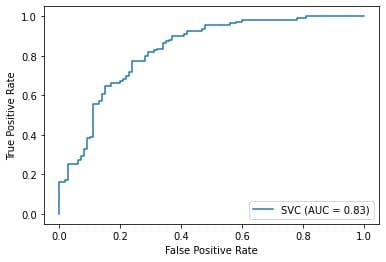
\includegraphics[width=\textwidth]{imgs/auc_svm.jpg}
            \caption[]{{\small SVM with kernel RBF}}    
        \end{subfigure}
        \hfill
        \begin{subfigure}[b]{0.475\textwidth}  
            \centering 
            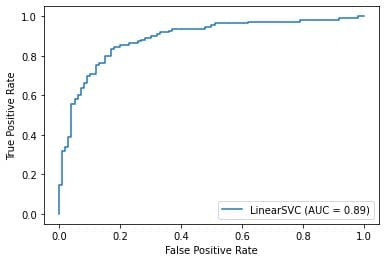
\includegraphics[width=\textwidth]{imgs/auc_linearsvm.jpg}
            \caption[]{{\small SVM with linear kernel}}    
        \end{subfigure}
        \vskip\baselineskip
        \begin{subfigure}[b]{0.475\textwidth}   
            \centering 
            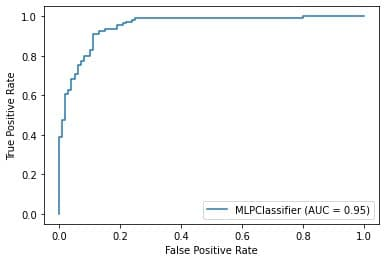
\includegraphics[width=\textwidth]{imgs/auc_MLP.jpg}
            \caption[]{{\small Multilayer Perceptron}}    
        \end{subfigure}
        \hfill
        \begin{subfigure}[b]{0.475\textwidth}   
            \centering 
            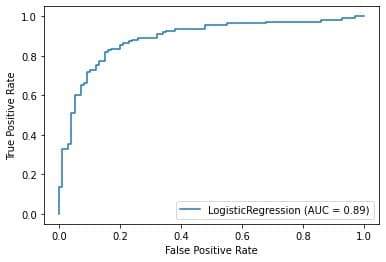
\includegraphics[width=\textwidth]{imgs/auc_LR.jpg}
            \caption[]{{\small Logistic regression}}    
        \end{subfigure}
        \caption[]{\small ROC graph of the best model of each family} 
        \label{fig:test_results}
    \end{figure*}


\subsection*{Other considered approaches.}

\begin{enumerate}
  \item Along with the landmark intensity, we made attempts where the landmark locations were used, this resulted in a clear overfitting. As a regularization approach, we centered those locations in order to make them image size-invariant. As a result the performance improved in Task 1 but lowered in Task 2.
  \item At one point, MTCNN and dlib did not return the face and landmarks for every image, at training we decided to skip that image it those features were not detected. However, this cannot be applied to test cases. We decided that, if given a test case we could not detect its features, we would assume it has the same features of a previous image of the same class. In the end, we needn't this but we are leaving all the code checks in case it is needed in the future.
  \item More models have been tested in the grid search, such as Random forests and other boosting techniques, however, they performed so poorly compared to the other models that we decided to not include them (decreasing the computational cost of the grid search).
\end{enumerate}

\section*{Task 2: inter-database analysis}

\textit{The goal of this task is to evaluate the DeepFake detection system developed in Task 1 with a new database (not seen during the development/training of the detector). In this task, you should use only the Celeb-DF. You only need to evaluate your fake detector developed in Task 1 over the \texttt{evaluation} dataset of Celeb-DF, not train again with them.}

\textbf{a)} \textit{Describe the results achieved by your DeepFake detection system developed in Task 1 using the evaluation dataset of the Celeb-DF database. Show the results achieved in terms of ROC curve and AUC. Provide an explanation of your results in comparison with the results of Task 1.}

As we said in the previous section, our considered model is the multilayer perceptron with the parameters achieved during the grid search. 

The model evaluation in the new dataset raises an AUC of 0.57166, this value is considerably lower than the ones achieved during the training phase, which makes sense considering that the first dataset from AUDFV was easier than this one from Celeb-DF in the sense that the deep fake was more easily spotted by an human. 


    \begin{figure*}
        \centering
        \begin{subfigure}[b]{0.475\textwidth}
            \centering
            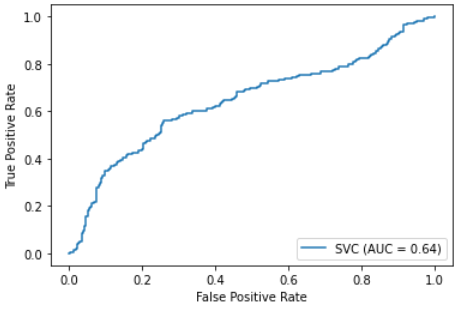
\includegraphics[width=\textwidth]{imgs/SVM_test.PNG}
            \caption[]{{\small SVM with kernel RBF}}    
        \end{subfigure}
        \hfill
        \begin{subfigure}[b]{0.475\textwidth}  
            \centering 
            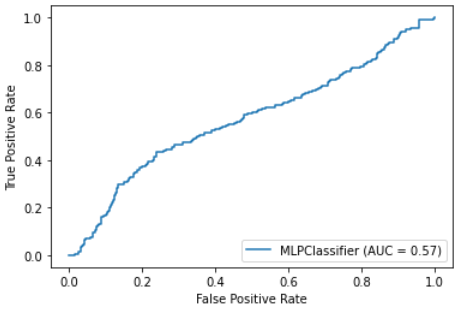
\includegraphics[width=\textwidth]{imgs/MLP_test.PNG}
            \caption[]{{\small Multilayer perceptron}}    
        \end{subfigure}
        \caption[]{\small ROC graph over Celeb-DF database} 
        \label{fig:test_celeb}
    \end{figure*}



In the training dataset there are usually vertical nad horizontal markings surrounding the face. In this new dataset, deepfakes have a higher quality and do not show such markings. In short, the selected model scales poorly to this dataset because the training model is not \textbf{representative} enough.


It is worth mentioning that even though we selected the perceptron as our testing model, we checked the performance of the other three. In this results, we saw that the SVM with RBF kernel achieved a \( 0.601 \) AUC. This means that the SVM model is the one that did the best at learning \emph{what a deep fake is} and did not overfit as much as the others.


\section*{Task 3: inter-database proposal}

\textit{The goal of this task is to improve the DeepFake detection system originally developed in Task 1 in order to achieve better inter-database results. You must consider the same evaluation dataset as in Task 2 (i.e. the \texttt{evaluation} dataset of the Celeb-DF database).}

\textbf{a)} \textit{Describe the improvements carried out in your proposed DeepFake detection system in comparison with Task 1.}

\textbf{b)} \textit{Describe the results achieved by your enhanced DeepFake detection system over the final evaluation dataset. Show the results achieved in terms of ROC curve and AUC. Provide an explanation of your results in comparison with the results of Task 2.}

\textbf{c)} \textit{Indicate the conclusions and possible future improvements}.

%%%%%%%%%%%%%%%%
%% Bibliography
%%%%%%%%%%%%%%%%

\bibliographystyle{authordate1}
\bibliography{bibliography}

\end{document}
